\documentclass[12pt]{article}
\usepackage[utf8]{inputenc}
\usepackage[pdftex]{graphicx}
\usepackage{graphicx}
\usepackage{geometry}
\usepackage{indentfirst}
\usepackage{setspace}
\usepackage{anysize}
\usepackage{makeidx}
\usepackage[brazil]{babel}
\usepackage{longtable}
\usepackage{multirow} 
\usepackage{hyperref}
\makeindex

\newcommand{\longtableendfoot}{Continuará na próxima página}

\geometry{
verbose,
a4paper,
left = 30mm,
top = 30mm,
right = 20mm,
bottom = 20mm
}

\begin{document}

\vbox{\Huge
%Nome do Trabalho
MANUAL DO JOGO SEVEN KEYS
%\ver
\vspace{0.03\textheight}
\hrule }
\section{Apresentação do jogo}
\subsection{Objetivo do documento}
O objetivo desse documento é apresentar as características principais do jogo 7 Keys, sua história, mecânicas e controles do jogo, para facilitar a interação do jogador com o jogo.

\subsection{Objetivo do jogo}     
O principal objetivo do jogo é fugir do santório. O jogador começa na ala de celas e precisa alcançar o térreo. Para finalizar cada fase será necessário encontrar uma chave específica que abra a porta que dá acesso ao andar inferior ou à próxima ala.

\subsection{Características gerais}

O jogo terá uma movimentação semelhante a games do estilo Legend of Zelda a Link to the Past e Fatal Labirinth como principais referências e exemplos os jogos The Binding of Isaac e Metal Gear Solid IV como referência para a mecânica de stealth.

 O jogo baseia-se em dois gêneros: stealth e roguelike. Stealth é um gênero onde o jogador precisa evitar ser notado, utilizando da furtividade para evadir ou elaborar emboscadas para os antagonistas. Jogos do gênero empregam mecânicas como se esconder na sombra, em objetos do cenário, disfarces, e barulhos que podem alertar os inimigos. Roguelike é um subgênero, geralmente de jogos de RPG, que é caracterizado pela geração de mapas aleatórios durante a partida, mapas baseados em tile e permanent death.

\section{A história do jogo}

   Início da 2a Guerra Mundial. A Alemanha invadiu a Polônia, levando a França e o Reino Unido a declarar guerra à Alemanha. O personagem, Edmond Gauthier - um sargento do exército francês - é um homem com um forte senso de honra que lidera bravamente seu exército frente ao inimigo alemão.
   
Em uma missão de resgate na Polônia, Edmond Gauthier e seu exército sofrem uma emboscada, planejada com o principal objetivo de impedi-los de resgatar os reféns judeus que seriam levados ao campo de concentração alemão ainda em construção. Embora a emboscada tenha causado algumas baixas, Edmond consegue alcançar os reféns, porém tarde demais. Ao se aproximar do local, ele percebe que os reféns já haviam sido executados e estavam sendo removidos do caminhão que continha a câmara de gás, uns dos últimos remanescentes da 1ª Guerra Mundial.
   
    Mesmo tendo falhado na missão, o exército francês ataca os alemães, numa espécie de revanche e  aprisiona-os. O superior de Edmond define então que os soldados nazistas aprisionados devem ser fuzilados, o que abala Edmond. Embora seja claro que os nazistas são um mal crescente, o código de honra de Edmond não o permite assassinar homens indefesos, sem a menor chance de revidarem ou sequer se protegerem. No entanto, como a ordem veio de um superior, Edmond é obrigado a obedecer e fuzila os nazistas aprisionados. Após essa missão mal sucedida, e com a crescente ameaça alemã, Edmond resolve voltar ao seu lar na França para se despedir de sua família e os mandarem para a Inglaterra, onde supostamente estariam mais protegidos.
    
    Em 1940, a Alemanha contorna a Linha Magnot - barreira de defesa que cobria toda a fronteira entre a França e a Alemanha, criada pela França após a 1a Guerra Mundial para evitar ataques surpresa e garantir mais tempo de resposta aos franceses em caso de um ataque frontal – vindo pelas densas florestas de Ardenas, único local desprotegido, pois acharam que os tanques alemães não conseguiriam atravessar a floresta. O General Weygand, recentemente nomeado, tomou ações imediatas para conter os alemães. Edmond então é enviado juntamente com o exército francês para conter os alemães. Durante a missão, Dante Chevalier, amigo de Edmond fica sob a mira do fogo inimigo. Edmond, logo parte em sua defesa, abatendo um soldado inimigo de pequeno porte. Ao investigar o corpo do inimigo, Edmond percebe que o soldado era uma criança, de aparentemente menos que 15 anos, o que o deixa perturbado. 
    
    Dois dias depois, ainda tentando conter os alemães, seu esconderijo é atacado por um tanque, desmoronando sobre suas cabeças. Edmond percebe então que Pierre ficou preso nos escombros. Ao tentar resgatar o amigo, acaba notando que o mesmo já se encontrava praticamente sem pulso e desacordado. Edmond decide então, mesmo contra sua vontade, abandonar o amigo e os demais soterrados e foi ao encalço dos alemães.
    
    O exército francês recua enquanto aguarda reforços e, ao receber informes da situação da Europa, descobre que a cidade inglesa onde sua família encontrava-se refugiada foi fortemente bombardeada pelos exércitos alemães. Esse era então o fim para Edmond Gauthier. Nada mais que ele amava lhe restava, além de amargas lembranças dos últimos e turbulentos meses. No entanto, uma missão mais precisava ser cumprida: parar os alemães.
    
    Os alemães, por outro lado, estavam muito fortalecidos e, mesmo com todo o empenho do exército francês e inglês, eles conseguiram avançar adentro do território francês. Edmond e mais alguns oficiais são então aprisionados e torturados em longos interrogatórios. Após obter as informações que necessitavam, os alemães aprisionaram os oficiais no campo de concentração de Bergen- Belsen (ou apenas Belsen) para utilizá-los depois como moeda de troca por oficiais alemães.
    
    Edmond não suporta a pressão causada pelas massivas perdas em sua vida e começa a agir de forma estranha, sendo constantemente atormentado pelas lembranças de seus entes queridos. Sendo considerado como louco, começa a receber uma série de medicações fortes que o deixa 'dopado' por meses a fio. A droga, que ainda estava em experimentação,  é tão forte que começa a afetar as lembranças de Edmond, que lentamente começa a se esquecer de todas as perdas bem como de quem ele próprio é, vivendo em um estágio próximo ao do vegetativo, apenas obedecendo ordens.
    
    Um dia, durante a manutenção do sistema de segurança do campo de concentração, uma pane ocorre no sistema elétrico e a segurança do complexo é comprometida. Praticamente todas as celas do complexo se destravam, o que causa uma tentativa de fuga em massa. Os guardas locais fazem o possível para conter os detentos, enquanto tentam comunicar-se com os campos próximos para solicitar reforços. Edmond, ainda meio sob o efeito dos medicamentos, tenta fugir também, sem atrair a atenção dos guardas. 
    
    Edmond precisará agora utilizar tudo que ainda se lembra para poder sobreviver. Isso significa se esconder nas sombras e atrás de objetos para evitar ser visto pelos guardas. Ou então, quando fugir do guarda não for opção, Edmond precisará eliminá-lo para prosseguir. O complexo em que ele se encontra possui 7 alas divididas em 3 andares, e para fugir ele precisará encontrar chaves específicas que dão acesso aos demais andares/alas até que ele alcance o salão central, que dá acesso aos jardins que por sua vez levam à uma densa floresta, possibilitando uma fuga mais “segura”.
    
    Além de lidar com os guardas, Edmond irá enfrentar outros seres, fantasmas que habitam sua mente. Esses fantasmas possuem características específicas que o relembram fatos importantes de sua vida. Esses fantasmas são, na verdade, suas lembranças de todas as mortes que o impactaram de alguma forma. No entanto, ele precisará lidar com essas lembranças e não só recordá-las como também aceitá-las para conseguir fugir do inferno em que se encontra. Caso contrário, ele será completamente consumido pela insanidade cada vez mais próxima dele, nesse ambiente completamente hostil e cheio de armadilhas, aguardando-o em cada sala. 

\section{Personagem Principal}
Edmond Gauthier, centro da trama do jogo, foi inspirado em soldados franceses que foram presos durante o início da Segunda Guerra Mundial e ficaram em campos de concentração para serem utilizados como moeda de troca. O personagem no início do jogo não consegue se lembrar direito de como ele foi parar naquele sanatório, por estar submetido à uma medicação forte o suficiente para afetar ainda mais a sua mente já deteriorada.

Durante todo o jogo o personagem mistura momentos de lucidez com momentos onde a loucura fala mais alto, que é quando os fantasmas surgem. Nas \textit{cutscenes} isso é mais evidente, onde a mente de Edmond oscila entre as recordações de seu passado, a realidade e a insanidade de sua mente, lutando contra seus fantasmas interiores à medida que tenta recuperar sua memória.

O personagem pode interagir com policiais que tentam conter os prisioneiros em fuga e com loucos que tentam fugir e matam quem encontrar pelo caminho. Ao encontrar um policial, o personagem poderá evitar entrar em seu campo de visão para não ser encontrado. Se o personagem escolher por assassinar o guarda, um fantasma do mesmo surgirá no local para atrapalhar o player, diminuindo sua vida e sanidade gradualmente à medida que permanece próximo à Edmond. Se encontrar um louco, ou o personagem deve tentar fugir o mais rápido possível ou abater o louco, já que o louco irá colocar sua vida em risco tão logo encontre Edmond.

\begin{figure}[h]
    \centering
    \caption{Concept art do Edmond}
     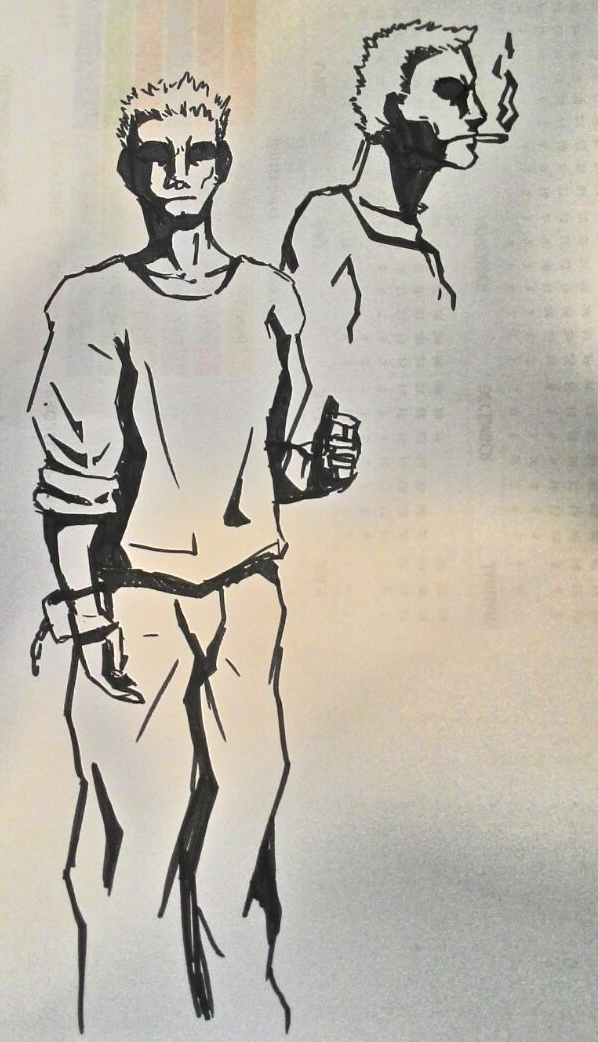
\includegraphics[keepaspectratio=true,scale=0.30]{GDD/images/Prev_Ed.png}
\end{figure}

\begin{figure}[h]
    \centering
    \caption{Imagem do Edmond \textit{in game}}
     
\includegraphics[keepaspectratio=true,scale=3]{GDD/images/e_ig.png}
\end{figure}

\vspace*{8cm}
\newpage
\section{Câmera e HUD}
A câmera do jogo é fixa e vista de um ângulo superior inclinado, mais conhecido como \lq\lq visão de pássaro\rq\rq. 

No canto superior esquerdo será apresentado as três barras de dados fundamentais do jogo na seguinte ordem: barra de vida, barra de resistência (stamina) e de sanidade. As barras estão alinhadas a uma imagem do rosto do player que irá variar de acordo com o nível da barra da sanidade.

No canto inferior esquerdo será apresentado os botões de ação do personagem que demonstram os itens que o player poderá utilizar, tanto para ataque quanto para se curar.

\begin{figure}[!h]
    \label{hud}
    \centering
    \caption{Câmera do HUD}
    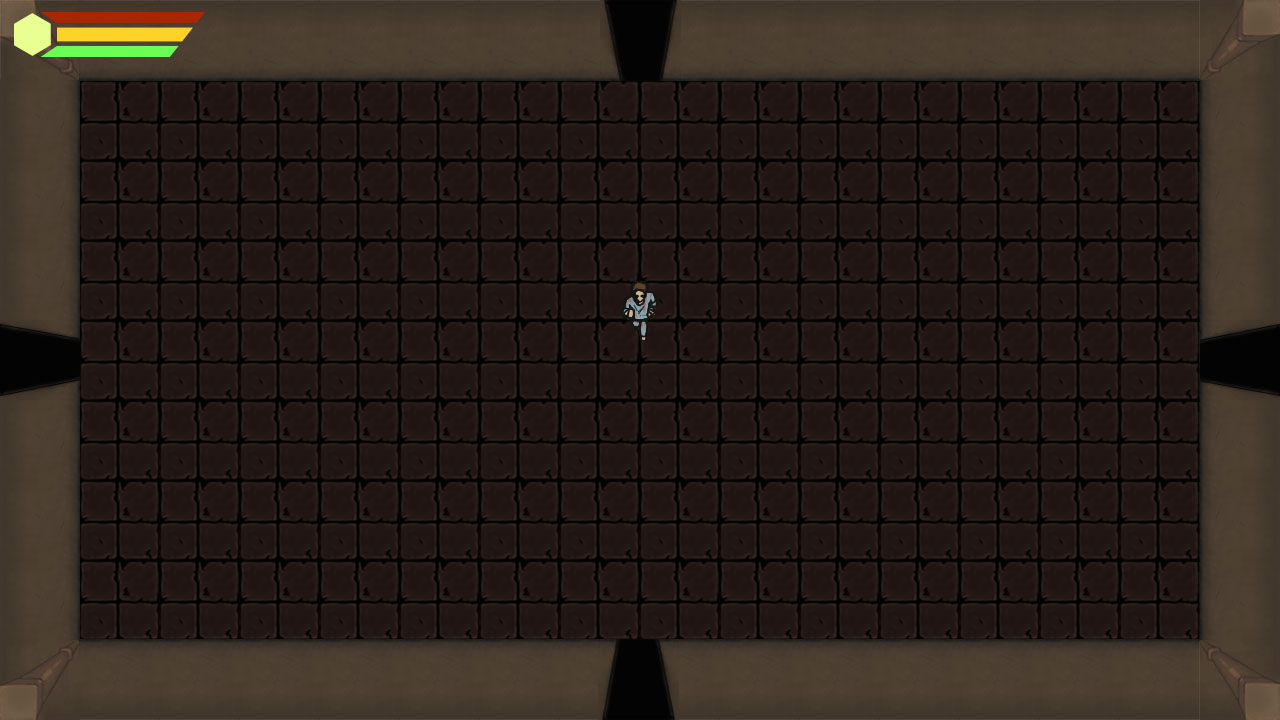
\includegraphics[keepaspectratio=true,scale=0.35]{GDD/images/HUD.jpg}
\end{figure}
\vspace*{7cm}

\section{\label{ctrl} Controles}
O jogador poderá usar como forma de controle para o jogo o teclado do computador. A tabela presente nessa seção apresenta as devidas funcionalidades presentes no jogo.

\begin{longtable}{|c|p{10cm}|}
\caption{Controles do jogo}
\onehalfspacing
\\
\hline
\multicolumn{2}{|c|}{Lista de comandos do jogo}
\\
\hline

\includegraphics[scale=0.3]{GDD/images/kW.png} 

\includegraphics[scale=0.3]{GDD/images/kA.png}

\includegraphics[scale=0.3]{GDD/images/kS.png}

\includegraphics[scale=0.3]{GDD/images/kD.png}
& Movimentar o personagem na tela
\\
\hline

\includegraphics[scale=0.3]{GDD/images/kL.png}
 & Correr (na direção selecionada)
\\
\hline

\includegraphics[scale=0.3]{GDD/images/kC.png}
& Agachar e andar agachado (pressionando algum botão direcional)
\\
\hline

\includegraphics[scale=0.3]{GDD/images/kH.png}
& Ataque com arma secundária
\\
\hline

\includegraphics[scale=0.3]{GDD/images/kJ.png}
& Ataque principal (No menu: selecionar opção)
\\
\hline

\includegraphics[scale=0.3]{GDD/images/kK.png}
& Interagir com itens (No menu: negar opção)
\\
\hline

\includegraphics[scale=0.3]{GDD/images/kQ.png}
& Usar item 
\\
\hline

\includegraphics[scale=0.3]{GDD/images/kE.png}
& Abre a porta especial (ao possuir a chave) 
\\
\hline

\includegraphics[scale=0.3]{GDD/images/kP.png}
& \textbf{Passa para a próxima fase (\textit{cheat})}
\\
\hline
\end{longtable}

\section{Instalação}

    Como o jogo ainda não possui instalador, o usuário deverá baixar o repositório do jogo \textit{Seven Keys} e compilar o mesmo, atualmente apenas para o sistema operacional linux.
    \subsection{Repositório}
        O repositório do jogo pode ser encontrado em: \textbf{https://github.com/ShutUpPaulo/ManaTeam}
    \subsection {Libs}
        Para tornar a compilção do jogo possível, o usuário deverá instalar as libraries da engine \textit{SDL2} e da engine \textit{IJE}.

        \subsubsection{SDL2}
            A seguir estão os comandos necessários para instalar as libraries da engine SDL2 no linux: sudo apt-get install libsdl2-dev libsdl2-mixer-dev libsdl2-image-dev libsdl2-ttf-dev

        \subsubsection{IJE}
            Para installar a engine IJE, primeiro é necessário baixá-la em seu repositório em \textbf{https://github.com/edsomjr/IJE/tree/7keys}, e, pelo terminal, acessar o a pasta em que foi baixada e rodar os comandos: \textit{make -j8}, depois \textit{sudo make install}.

        \subsubsection{Compilando o jogo Seven Keys}
            Após instalada as duas engines, basta ir para a pasta ~/Manateam/Game/ e rodar o comando: \textit {make -j8}.
            O executavel binário estará na pasta \textit{~Manateam/Game/bin/}.


\end{document}